
\chapter{Resultat}

\begin{binge}

\section{Läromaterialet}

Läromaterialet blev i slutändan, precis som målet var, en sammanvävning mellan domänspecifika språk som modellerar fysik och brödtext som förklarar både fysiken i sig, men också förklarar de domänspecifika språken.

\begin{figure}
  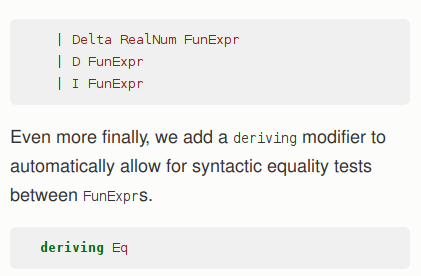
\includegraphics[width=\linewidth]{figure/smakprov_laromaterial.png}
  \caption{Ett smakprov över hur det resulterande läromaterielt ser ut.}
  \label{fig:smakprov_läromaterial}
\end{figure}

Figur \ref{fig:smakprov_läromaterial} visar ett smakprov över det resulterande läromaterialet. Som figuren visar är brödtext sammanvävt med Haskell-kod för domänspecifika språk.

Läromataterialet behandlar ett flertal områden inom fysik, samt matematik som används inom fysik. Fokuset är på mekanik samt till det området tillhörande matematik. I sin fullständighet är de behandlade områdena

\begin{itemize}
  %\setlength\itemsep{-12pt}
  \item Analys
  \item Bevis
  \item Dimensioner
  \item Fysikaliska kroppar
  \item Vektorer
\end{itemize}

\textit{Analys} handlar om matematisk analys och bygger upp ett syntaxträd... TODO: kolla mer detaljrikt.

I \textit{Bevis}-kapitlet presenteras bevisföringen med hjälp av Haskells typsystem. Det exemplifieras genom att kinematiska formler bevisas.

\textit{Dimensioner} behandlar dimensioner, storheter och enheter inom fysiken. Dimensioner införs på typnivå i Haskell för att kunna visa på likheten mellan Haskells typsystem och hur man måste förhålla sig till dimensioner inom fysiken.

\textit{Fysikaliska kroppar} vet ej TODO: ta reda på

\textit{Vektorer} vet ej TODO: ta reda på

I läromataterialet finns, förutom de fem ovanstående separata områdena, även tillämpningar av de områdena på exempelproblem. Till exempel används \textit{Dimensioner} till att lösa problem med fritt fall. TODO: fyll på när vet mer om hur tillämpningarna ser ut.

\subsection{Domänspecifika språk}

De domänspecika språken är avgränsade och behandlar separata områden. De är avgränsade för att det är enklare att förstå dem om de är det. Av samma skäl behandlar de separata områden. Om det skulle uppstå behov kan de kombineras istället.

De domänspecifika språken modellerar områden snarare än att vara problemlösare. \textit{Analys} exemplifierar detta väl. Det språket består av ett syntaxträd över algebraiska uttryck samt operationer som derivering och integration. Med hjälp av det kan man modellera uttryck och analytiska operationer på dem. Däremot löser det inte problem åt en. Man kan med andra ord inte mata in en differentialekvation och automatiskt få en lösning.

TODO: Detta kanske passar bättre i diskussion: Hur bra våra moduler blev samt varför de inte är problemlösare utan modellerare istället.

\subsection{Brödtexten}

Brödtexten finns till som ett förklarande komplement till de domänspecifika språken. Texten förklarar dels den bakomliggande fysiken, dels den Haskell-kod som finns. Generellt står förklaring av kod för en stor del av brödtexten. Detta för att det är själva modellerandet som är den stora delen - det är egentligen ganska lite fysik som presenteras. Därav behöver koden en utförlig förklaring. Dessutom används avancerade koncept i Haskell, bland annat typnivå-programmering, som läsaren inte förväntas kunna sedan innan. Av naturliga skäl kräver dessa en längre förklaring.

Texten är skriven på engelska för att komma fler till gagn än om den varit skriven på svenska.

Språket i texten är vardagligt och lättsamt. Detta för att vara en kontrast mot hur kursböcker vanligtvis ser ut.

I brödtexten finns bilder. De har en rolig och medvetet kladdig stil. Syftet är att muntra upp läsaren. Figur \ref{fig:smakprov_bild_laromaterial.png} är ett exempel på en bild som finns i läromaterielet. Den visar den humoristiska och oseriösa ritningstekniken.

\begin{figure}
  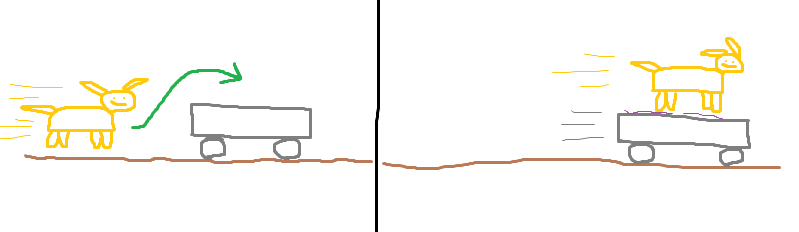
\includegraphics[width=\linewidth]{figure/smakprov_bild_laromaterial.png}
  \caption{Exempel på bild ur läromaterilet}
  \label{fig:smakprov_bild_läromaterial}
\end{figure}

Valet att skriva på engelska, den lättsamma stilen och de roliga bilderna har inspirerats av *Learn You a Haskell*. TODO: referens. Läromaterialet är tänkt att vara något liknanden, men för fysik istället för Haskell.

TODO: Blev det en bra text? Kanske ska vara i diskussionen istället

\section{Hemsidan}

Läromaterialet finns tillgängligt på en hemsida, som består av grundläggande HTML, CSS och javascript. På hemsidan finns en innehållsförteckning med klickbara länkar till de olika kapitlen. Hemsidan är öppen för alla och bör fungera i de flesta webläsare.

\section{Källkod}

I projektbeskrivningen stod det att all källkod skulle finnas fritt tillgänglig. Det gör den också. Det finns tillgänglig på internet på projektes GitHub-repository TODO: referens.

Källkoden som finns är all den som använts under projekets gång, både slutversion och alla mellanversioner sedan projekets början. Källkoden är inte bara läromaterialet i sig, utan även kod till hemsidan, rapporter (inklusive denna) och mötesprotokoll.

\section{Återkoppling från testgrupp}

För att utvärdera huruvida läromaterialet är intressant och hjälpsamt har vi haft en informell återkoppling med en testgrupp. TODO: Skriv mer när vi faktiskt gjort detta.

\end{binge}
